\documentclass[a4paper,12pt]{article} % тип документа

% Поля страниц
\usepackage[left=2.5cm,right=2.5cm,
    top=2cm,bottom=2cm,bindingoffset=0cm]{geometry}
    
%Пакет дял таблиц   
\usepackage{multirow} 
    
%Отступ после заголовка    
\usepackage{indentfirst}

% % Рисунки
% \usepackage{floatrow,graphicx,calc}
% \usepackage{wrapfig}

% %%% Работа с картинками
\usepackage{graphicx}  % Для вставки рисунков
% \graphicspath{{images/}{images2/}}  % папки с картинками
% \setlength\fboxsep{3pt} % Отступ рамки \fbox{} от рисунка
% \setlength\fboxrule{1pt} % Толщина линий рамки \fbox{}
% \usepackage{wrapfig} % Обтекание рисунков и таблиц текстом

% Создаёем новый разделитель
% \DeclareFloatSeparators{mysep}{\hspace{1cm}}

% % Ссылки?
% \usepackage{hyperref}
% \usepackage[rgb]{xcolor}
% \hypersetup{				% Гиперссылки
%     colorlinks=true,       	% false: ссылки в рамках
% 	urlcolor=blue          % на URL
% }


% %  Русский язык
% \usepackage[T2A]{fontenc}			% кодировка
% \usepackage[utf8]{inputenc}			% кодировка исходного текста
% \usepackage[english,russian]{babel}	% локализация и переносы
%%% Работа с русским языком
\usepackage{cmap}                           % поиск в PDF
\usepackage{mathtext} 			 	       % русские буквы в формулах
\usepackage[T2A]{fontenc}               % кодировка
\usepackage[utf8]{inputenc}              % кодировка исходного текста
\usepackage[english,russian]{babel}  % локализация и переносы


% Математика
% \usepackage{amsmath,amsfonts,amssymb,amsthm,mathtools}

%%% Дополнительная работа с математикой
% \usepackage{amsmath,amsfonts,amssymb,amsthm,mathtools} % AMS
% \usepackage{icomma} % "Умная" запятая: $0,2$ --- число, $0, 2$ --- перечисление


% Что-то 
% \usepackage{wasysym}

% Мое
% \usepackage{longtable}
% \usepackage{booktabs}


\begin{document}

\begin{center}   
	\large{Лабораторная работа № 2.5.1\\\textbf{Измерение коэффициента поверхностного натяжения жидкости}}\\
\end{center}

\section{Аннотация}

% \subparagraph*{Цель работы:} 1) измерение температурной зависимости  коэффициента поверхностного натяжения дистиллированной воды с использованием известного коэффициента поверхностного натяжения спирта;  2) определение полной поверхностной энергии  и теплоты, необходимой для изотермического образования единицы  поверхности жидкости  при различной температуре. 
% \subparagraph*{В работе используются:}прибор Ребиндера  с термостатом и микроманометром; исследуемые жидкости; стаканы.

	\noindent\textbf{Цель работы:}
	1) измерение температурной зависимости  коэффициента поверхностного натяжения дистиллированной воды с использованием известного коэффициента поверхностного натяжения спирта; 2) определение полной поверхностной энергии  и теплоты, необходимой для изотермического образования единицы  поверхности жидкости  при различной температуре.
	
	\bigskip
	\noindent\textbf{В работе используются:} прибор  Ребиндера  с термостатом и микроманометром; исследуемые жидкости; стаканы; микроскоп.

\section{Теоретические сведения}

Наличие поверхностного слоя приводит к различию давлений по разные стороны от искривленной границы раздела двух сред.  Для сферического пузырька с воздухом  внутри жидкости избыточное давление даётся формулой Лапласа:

\begin{equation}
\Delta P = P_{внутри}- P_{снаружи}=\frac{2\sigma}{r}, 
\end{equation}
где $\sigma$ -- коэффициент поверхностного натяжения, $P_{внутри}$ и $Р_{снаружи}$ -- давление внутри пузырька и снаружи, $r$ -- радиус кривизны поверхности раздела двух фаз. Эта формула лежит в основе предлагаемого метода определения коэффициента поверхностного натяжения жидкости. Измеряется давление $\Delta P$, необходимое для выталкивания в жидкость пузырька воздуха.

% \section{Методика измерений}

\newpage
\section{Используемое оборудование}

\begin{figure}[h!]
\begin{center}
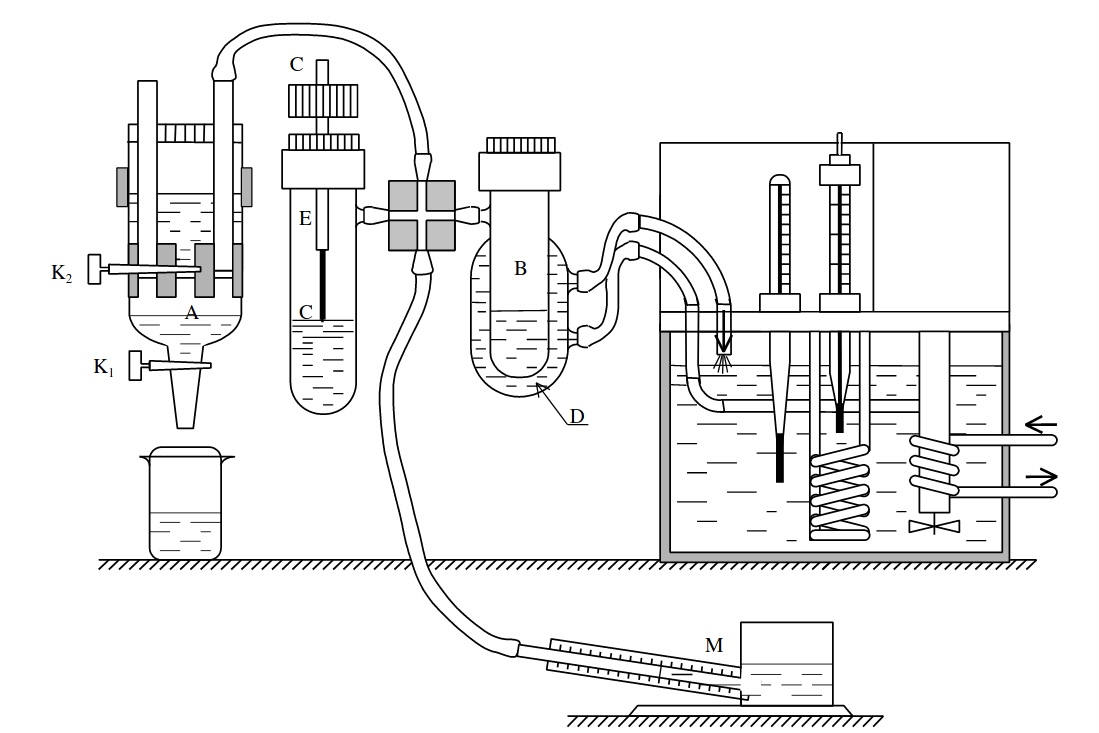
\includegraphics[width=\textwidth]{установка.jpg}
\end{center}
\caption{Схема установки} \label{установка}
\end{figure}

Схема экспериментальной установки представлена на рисунке \ref{установка}.
Тестовая жидкость (этиловый спирт) наливается в сосуд, через пробку в него входит полая металлическа игла. При создании достаточно разреженного воздуха в колбе пузырьки воздуха начинают пробулькивать, поверхностное натяжение измеряется по величине разряжения. Разряжение создается с помощью аспиратора, разность давлений измеряется спиртовым микроманометром.

Для стабилизации температуры через рубашку колбы с исследуемой жидкостью прогоняется вода из термостата. Из-за большой теплопроводности трубки температура в разных частях трубки заметно различна и ввиду теплового расширения поднимается уровень жидкости при изменении температуры. Поэтому при температурном измерениии кончик иглы опускают до самого дна сосуда, тогда:
\begin{equation}
\Delta P = P - \rho g h
\end{equation}
$\rho$ - плотность жидкости, $h$ - высота погружения иглы.


% \section{Результаты измерений и обработка данных}
% \section{Обсуждение результатов}
% \section{Заключение}

\end{document}